\section{Dispersal-Extinction-Cladogenesis model}

\subsection{Range characters}

Discrete biogeographical models typically rely on presence-absence data, where a species is observed or not observed across multiple discrete areas.
For example, say there are three areas: A, B, and C.
Say a species is present in areas A and C, then its range equals AC, which can also be encoded into the length-3 bit vector, 101.
Bit vectors may also be transformed into (decimal) integers, \EG the binary number 101 equals the decimal number 5.
\[
( \emptyset, A, B, AB, C, AC, BC, ABC ) \Leftrightarrow (000,100,010,110,101,011,111) \Leftrightarrow ( 0, 1, 2, 3, 4, 5, 6, 7 )
\]
Decimal representation is rarely used in discussion, but it is useful to keep in mind when considering the total number of possible ranges for a species.

\subsection{Modeling anagenic range evolution}

How might we model the dynamics of species range evolution?
In this section, we'll cover the Dispersal-Extinction-Cladogenesis model proposed by \citet{Ree2005}.
To begin, we'll focus on anagenesis: evolution that occurs between speciation events within lineages.
Since we have discrete characters we'll use the continuous-time Markov chain, which allows us to compute transition probability of a character changing from $i$ to $j$ in time $t$ through matrix exponentiation
\[
\mathbf{P}_{i,j}(t) = \left[ \exp \left\lbrace \mathbf{Q}t \right\rbrace \right]_{i,j},
\]
where $\textbf{Q}$ is the instantaneous rate matrix defining the rates of change between all pairs of characters, and $\textbf{P}$ is the transition probability rate matrix.
Remember, $i$ and $j$ represent different ranges, each of which is encoded as the set of areas occupied by the species.
Exponentiation of the rate matrix is powerful because it integrates over all possible scenarios of character transitions that could occur during $t$ so long as the chain begins in state $i$ and ends in state $j$.

We can then encode ${\bf Q}$ to reflect the allowable classes of range evolution events with biologically meaningful parameters.
We'll take a simple model of range expansion (e.g. $BC \rightarrow ABC$) and range contraction (e.g. $BC \rightarrow C$).
(Range expansion may also be referred to as dispersal or area gain and range contraction as extirpation, (local) extinction, or area loss.)
The rates in the transition matrix for three areas might appear as

\[
\textbf{Q} = 
	\begin{array}{c|cccccccc}
		& \emptyset & A & B & AB & C & AC & BC & ABC \\
		\hline
		\emptyset 	& - 	& 0 	& 0 	& 0 		& 0			& 0 		& 0 		& 0 \\
		A 			& e_A 	& - 	& 0 	& d_{AB} 	& 0			& d_{AC} 	& 0 		& 0 \\
		B 			& e_B 	& 0 	& - 	& d_{BA}	& 0			& 0 		& d_{BC} 	& 0 \\
		AB 			& 0 	& e_A 	& e_B 	& - 		& 0			& 0 		& 0 		& d_{AC} + d_{BC} \\
		C 			& e_C 	& 0 	& 0 	& 0 		& - 		& d_{CA} 	& d_{CB} 	& 0 \\
		AC 			& 0 	& e_C 	& 0 	& 0 		& e_A		& - 		& 0 		& d_{AB} + d_{CB} \\
		BC 			& 0 	& 0 	& e_C 	& 0 		& e_B		& 0 		& - 		& d_{BA} + d_{CA} \\
		ABC 		& 0 	& 0 	& 0 	& e_C 		& 0 		& e_B 		& e_A 		& - \\								
	\end{array},
\]
where $e = ( e_A, e_B, e_C )$ are the (local) extinction rates per area, and $d = ( d_{AB}, d_{AC}, d_{BC}, d_{CB}, d_{CA}, d_{BA})$ are the dispersal rates between areas.
Notice that the sum of rates leaving state $\emptyset$ is zero, meaning any species that loses all areas in its range remains permanently extinct.


{\bf \framebox{?} For the three-area DEC rate matrix above, what is the rate of leaving state AC in terms of dispersal and extinction parameters?}

Note the rate of more than one event occurring simultaneously is zero, so a range must expand twice by one area in order to expand by two areas.

{\bf \framebox{?} What series of transition events might explain a lineage evolving from range $ABC$ to range $A$? From range $AB$ to range $C$?}

Of course, this model can be specified for more than three areas.

{ \bf \framebox{?} Imagine a DEC rate matrix with four areas, $ABCD$. What would be the dispersal rate for $Q_{BC,BCD}$? How many states does a DEC rate matrix with four areas have? What is the relationship between the number of areas and the number of states under the DEC model? }

Let's consider what happens to the size of \textbf{Q} when the number of areas, $N$, becomes large.
For three areas, \textbf{Q} is size $8 \times 8$.
For ten areas, \textbf{Q} is size $2^{10} \times 2^{10} = 1024 \times 1024$, which approaches the largest size matrices that can be exponentiated in a practical amount of time.
For twenty areas, \textbf{Q} is size $2^{20} \times 2^{20} \approx 10^6 \times 10^6$ and exponentiation is not viable.


\subsection{Modeling cladogenic range evolution}

Cladogenesis describes evolutionary change accompanying speciation.
Daughter species are not expected to inherit their ancestral range identically in general.
For each internal node in the reconstructed tree, one of two cladogenic events can occur: sympatry or allopatry.
Say the range of a species is $A$ the moment before speciation occurs at an internal phylogenetic node.
Since the species range is size one, both daughter lineages necessarily inherit the ancestral species range ($A$).
In DEC parlance, this is called a {\it narrow sympatry} event.

Now suppose the ancestral range is $ABC$.
Under {\it subset sympatric cladogenesis}, one lineage identically inherits the ancestral species range, $ABC$, while the other lineage inherits only a single area, i.e. only $A$ or $B$ or $C$.
For {\it widspread sympatric cladogenesis}, both lineages inherit the ancestral range, $ABC$.
Under {\it allopatric cladogenesis}, the ancestral range is split evenly among daughter lineages, e.g. one lineage may inherit $AB$ and the other inherits $C$.

For an excellent overview of described state transitions for cladogenetic events, see \citet{Matzke2012}.

{\bf \framebox{?} Given the state is $AB$ before cladogenesis, and allowing subset sympatry, widespread sympatry, and allopatry, what are the 7 possible states in the daughter lineages after cladogenesis?}

The probabilities of anagenic change along lineages must account for all combinations of starting states and ending states.
For 3 areas, there are 8 states, and thus $8 \times 8 = 64$ probability terms for pairs of states.
For cladogenic change, we need transition probabilities for all combinations of states before cladogenesis, after cladogenesis for the left lineage, and after cladogenesis for the right lineage.
Like above, for three areas, there are 8 states, and $8 \times 8 \times 8 = 512$ cladogenic probability terms.

{\bf \framebox{?} For three areas, there are three narrow, four widespread, 18 subset sympatric events and 12 allopatric cladogenesis events. What proportion of terms in the cladogenesis matrix are zero?}

The DEC model ignores speciation events hidden by extinction or incomplete taxon sampling.
The probability of cladogenesis and local extinction events would ideally be linked to a birth-death process, as it is in the GeoSSE model \citep{Goldberg2011}.
Unfortunately, since the numerical method for SSE models scale poorly, and DEC models remain the only option when the geography has more than two or three areas.
For more than ten areas, data augmentation may be used to infer ancestral ranges, as described in Section \ref{sec:bayarea}.

%\begin{figure}[H]
%\centering
%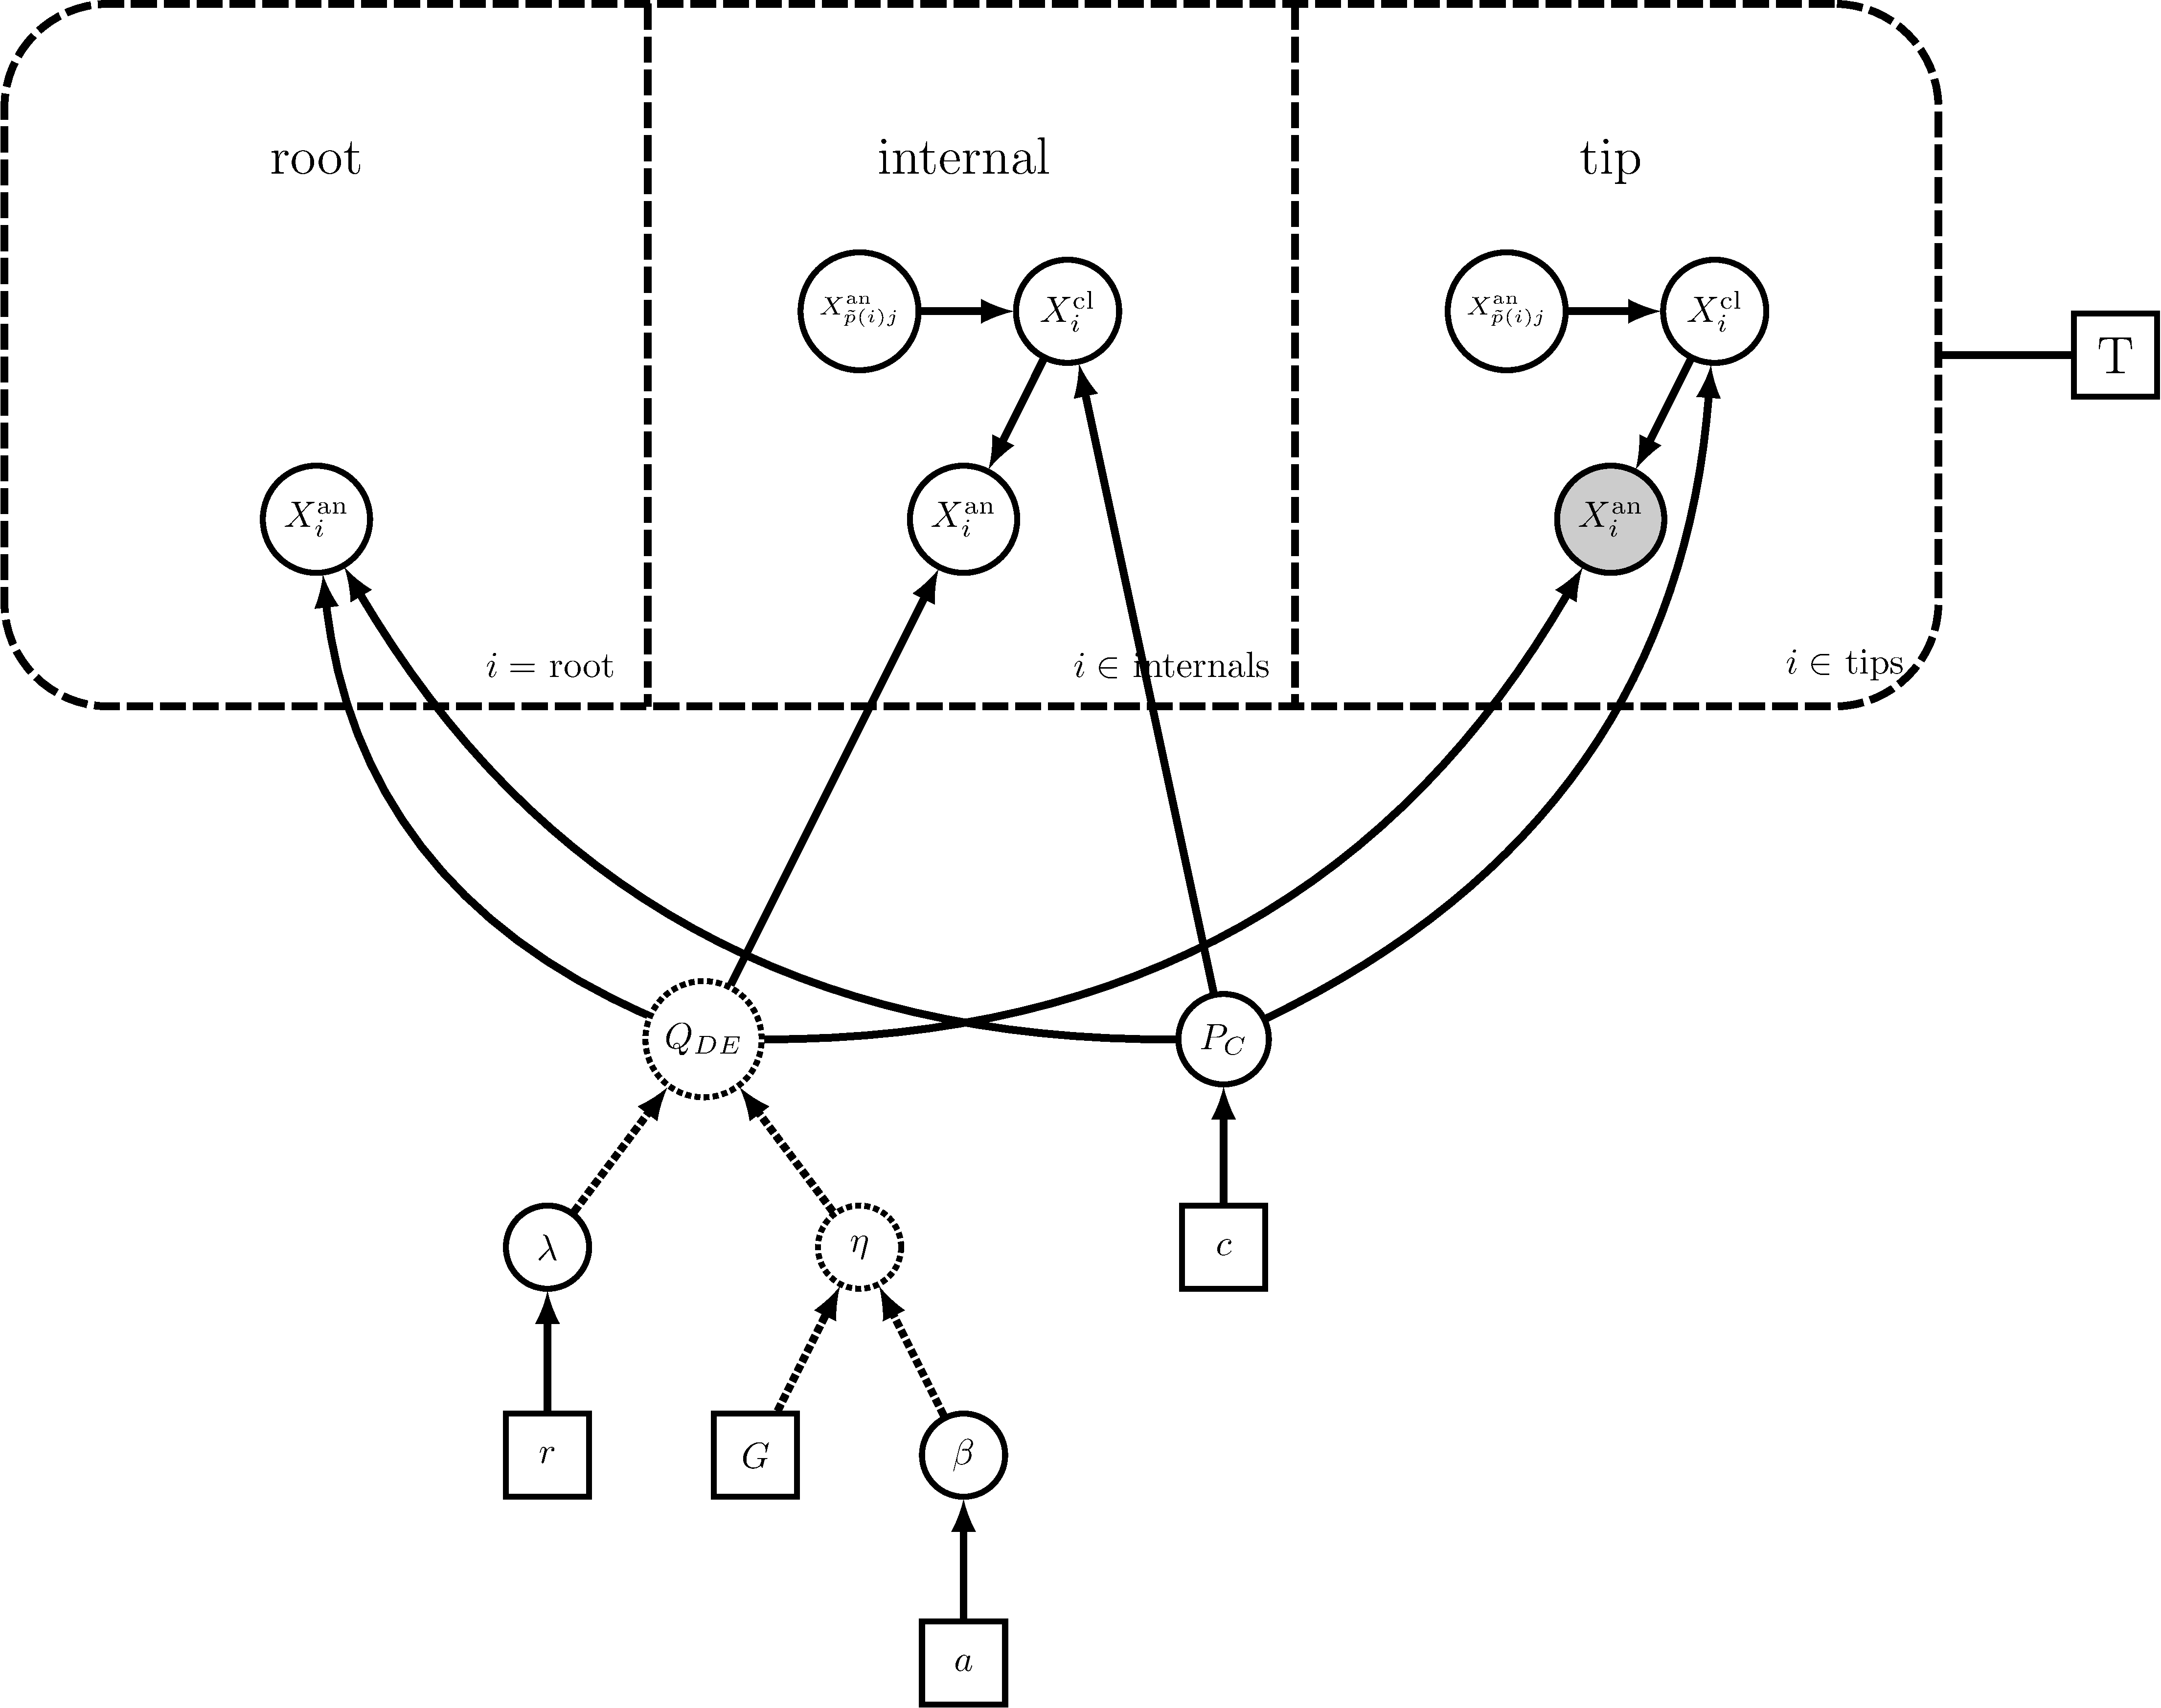
\includegraphics[width=5in]{figures/bg_dec_dag}
%\caption{Graphical model of DEC. The tree plate's topology is fixed by $T$, where each internal node has both an anagenic and cladogenic random variable ($X_i^{\text{an}}$ and $X_i^{\text{cl}}$, resp.) that represents an ancestral species before and after it speciated. Anagenic change is modeled by a continuous time Markov process, where $Q_{DE}$ is the instantaneous rate matrix of area gain and loss, as parameterized by $\lambda$. The geographic distance rate modifier function, $\eta$, takes in the geographical distances and strata as $G$, and the distance power parameter, $\beta$. Cladogenic change is modeled by $P_C$, a Dirichlet-distributed simplex with a flat prior.}
%\end{figure}

The rest of this section will describe how to run a simple DEC analysis using RevBayes.

\newpage
